\documentclass[10pt]{article} % For LaTeX2e
\usepackage{tmlr}
% If accepted, instead use the following line for the camera-ready submission:
%\usepackage[accepted]{tmlr}
% To de-anonymize and remove mentions to TMLR (for example for posting to preprint servers), instead use the following:
%\usepackage[preprint]{tmlr}

% amsthm
\newtheorem{proposition}{Proposition}
% \newtheorem*{proposition*}{Proposition}
\newtheorem{corollary}{Corollary}
% \newtheorem*{corollary*}{Corollary}
\newtheorem{definition}{Definition}
% \newtheorem{claim}{Claim}
% \newtheorem{question}{Question}


% probability theory
% \newcommand{\expect}{\mathbbm{E}}
% \newcommand{\prob}{\mathrm{P}}
% \newcommand{\Var}{\operatorname{Var}}
% \newcommand{\Cov}{\operatorname{Cov}}
% \newcommand{\Erf}{\operatorname{Erf}}
% \newcommand{\Erfc}{\operatorname{Erfc}}
\newcommand{\Pp}{\operatorname{P}}

% \newcommand{\boxx}[1]{\fbox{\parbox{\columnwidth}{#1}}}

% aliases
% \newcommand{\f}{\mathfrak}
% \newcommand{\mc}{\mathcal}
% \newcommand{\mb}{\mathbf}

% symbols
% \newcommand{\tail}{\overline{F}}
% \newcommand{\sign}{\operatorname{sign}}
% \newcommand{\op}{\operatorname{op}}
% \newcommand{\pr}{\operatorname{pr}}
% \newcommand{\adj}{\operatorname{adj}}
% \newcommand{\sgn}{\operatorname{sgn}}
% \newcommand{\xb}{{\mathbf x}}
% \newcommand{\vb}{{\mathbf v}}
% \newcommand{\Lie}{{\mathcal L}}
% \newcommand{\deq}{\stackrel{\text{def}}{=}}
% \newcommand{\eps}{\epsilon}
% \newcommand{\Ci}{{C^\infty}}
% \newcommand{\Id}{\operatorname{Id}}
% \newcommand{\lexp}{\overleftarrow{\exp}}
% \newcommand{\rexp}{\overrightarrow{\exp}}
% \newcommand{\One}{\mathbbm{1}}
% \newcommand{\Two}{\mathbbm{2}}
% \newcommand{\ot}{\leftarrow}
% \newcommand{\brak}[1]{\langle #1 \rangle}
% \newcommand{\bbrak}[1]{\llangle #1 \rrangle}
% \newcommand{\relat}[1]{\stackrel{#1}{\sim}}
% \newcommand{\mx}{\hat{\f m}}
% \newcommand{\Sb}{\operatorname{Sb}}
% \newcommand{\SO}{\operatorname{SO}}
% \newcommand{\LO}{\operatorname{O}}
% \newcommand{\ad}{\operatorname{ad}}
% \newcommand{\Ad}{\operatorname{Ad}}
% \newcommand{\Ac}{\mathcal{A}}
% \newcommand{\F}{\mathcal{F}}
% \newcommand{\so}{\mathfrak{so}}
% \newcommand{\Fc}{\mathcal{F}}
% \newcommand{\Xc}{\mathcal{X}}
% \newcommand{\Yc}{\mathcal{Y}}
% \newcommand{\E}{\operatorname{E}}
% \providecommand{\P}{\mathbb{P}}
% \newcommand{\Pc}{\mathcal{P}}
% \newcommand{\Sc}{\mathcal{S}}
% \newcommand{\ddtz}{{\left (\frac d {dt} \right)_0}}
% \newcommand{\Cc}{\mathcal{C}}
% \newcommand{\Xcal}{\mathcal{X}}
% \newcommand{\Rcal}{\mathcal{R}}
% \newcommand{\ptimes}{{\otimes p}}
% \newcommand{\Vc}{\mathcal{V}}
% \newcommand{\vspan}{\operatorname{span}}
\newcommand{\R}{\mathbb{R}}
\newcommand{\C}{\mathbb{C}}
\newcommand{\K}{\mathbb{K}}
\newcommand{\T}{\mathbb{T}}
% \newcommand{\GL}{\operatorname{GL}}
% \newcommand{\gl}{\f{gl}}
% \newcommand{\End}{\operatorname{End}}
% \newcommand{\Aut}{\operatorname{Aut}}
% \newcommand{\N}{\mathbb{N}}
% \newcommand{\Hom}{\operatorname{Hom}}
% \newcommand{\im}{\operatorname{im}}
% \newcommand{\Or}{\mathcal{O}}
% \newcommand{\Div}{\operatorname{div}}
% \newcommand{\tr}{\operatorname{tr}}
% \newcommand{\Z}{\mathbb{Z}}
% \newcommand{\Q}{\mathbb{Q}}
% \newcommand{\Sp}{\mathbb{S}}
% \newcommand{\Frac}{\operatorname{frac}}
% \newcommand{\Pp}{\operatorname{P}}
% \newcommand{\Le}{\mathcal{L}}
% \newcommand{\id}{{\operatorname{id}}}
% \newcommand{\diam}{\operatorname{diam}}
% \newcommand{\norm}[1]{{\left\lVert{#1}\right\rVert}}
% \newcommand{\abs}[1]{{\left\lvert{#1}\right\rvert}}
% \newcommand{\aseq}{\stackrel{\text{a.s.}}{=}}
% \newcommand{\rank}{\operatorname{rank}}
% \newcommand{\Gr}{\operatorname{G}}


\usepackage{hyperref}
\usepackage{url}
\usepackage{amsmath}
\usepackage{amssymb}
\usepackage{cleveref}
\usepackage{graphicx}

\title{How Much Information Fits in a Vector?}

\author{\name Christopher Gadzinski \email christopher.gadzinski@uni.lu \\
      \addr Department of Computer Science\\
      University of Luxembourg}

\newcommand{\fix}{\marginpar{FIX}}
\newcommand{\new}{\marginpar{NEW}}

\def\month{10}  % Insert correct month for camera-ready version
\def\year{2025} % Insert correct year for camera-ready version
\def\openreview{\url{https://openreview.net/forum?id=XXXX}}

\begin{document}

% \maketitle

\begin{abstract}
Recent work in neural network interpretability has posited that hidden activations of some deep models can be viewed as superpositions of sparsely activated ``feature vectors.'' In general, this kind of representation is known as a superposition code. This work presents an information-theoretic account of superposition codes in a setting intended to model applications of SAEs. We show that, when the number $k$ of active features is very small compared to the number $N$ of total possible features, surprisingly simple superposition methods can encode and decode these representations provided that $d$ is a constant factor greater than the Shannon limit. Specifically, when $\ln k / \ln N \le \epsilon < 1,$ it suffices that $C(\eta) d \ge H,$ where $H$ is the entropy to be transmitted and $C(\eta)$ is a certain decreasing function of $\eta.$. However, the maximum value of $d/H$ varies significantly depending on the decoding method used. For example, under moderate values of $\eta,$ we find that certain natural decoding methods are limited to transmission rates of less than $1/6$ bits per dimension. On the other hand, we show empirically that a cheap iterative method can achieve around $3/4$ bits per dimension. Our results address a lack of practical references on superposition codes in a very sparse regime and provide a possible information-theoretic explanation for the limited success of SAEs.
\end{abstract}

\section{Introduction}

\begin{figure}[b]
	\begin{minipage}[c]{0.5\textwidth}
		\begin{center}
		\centerline{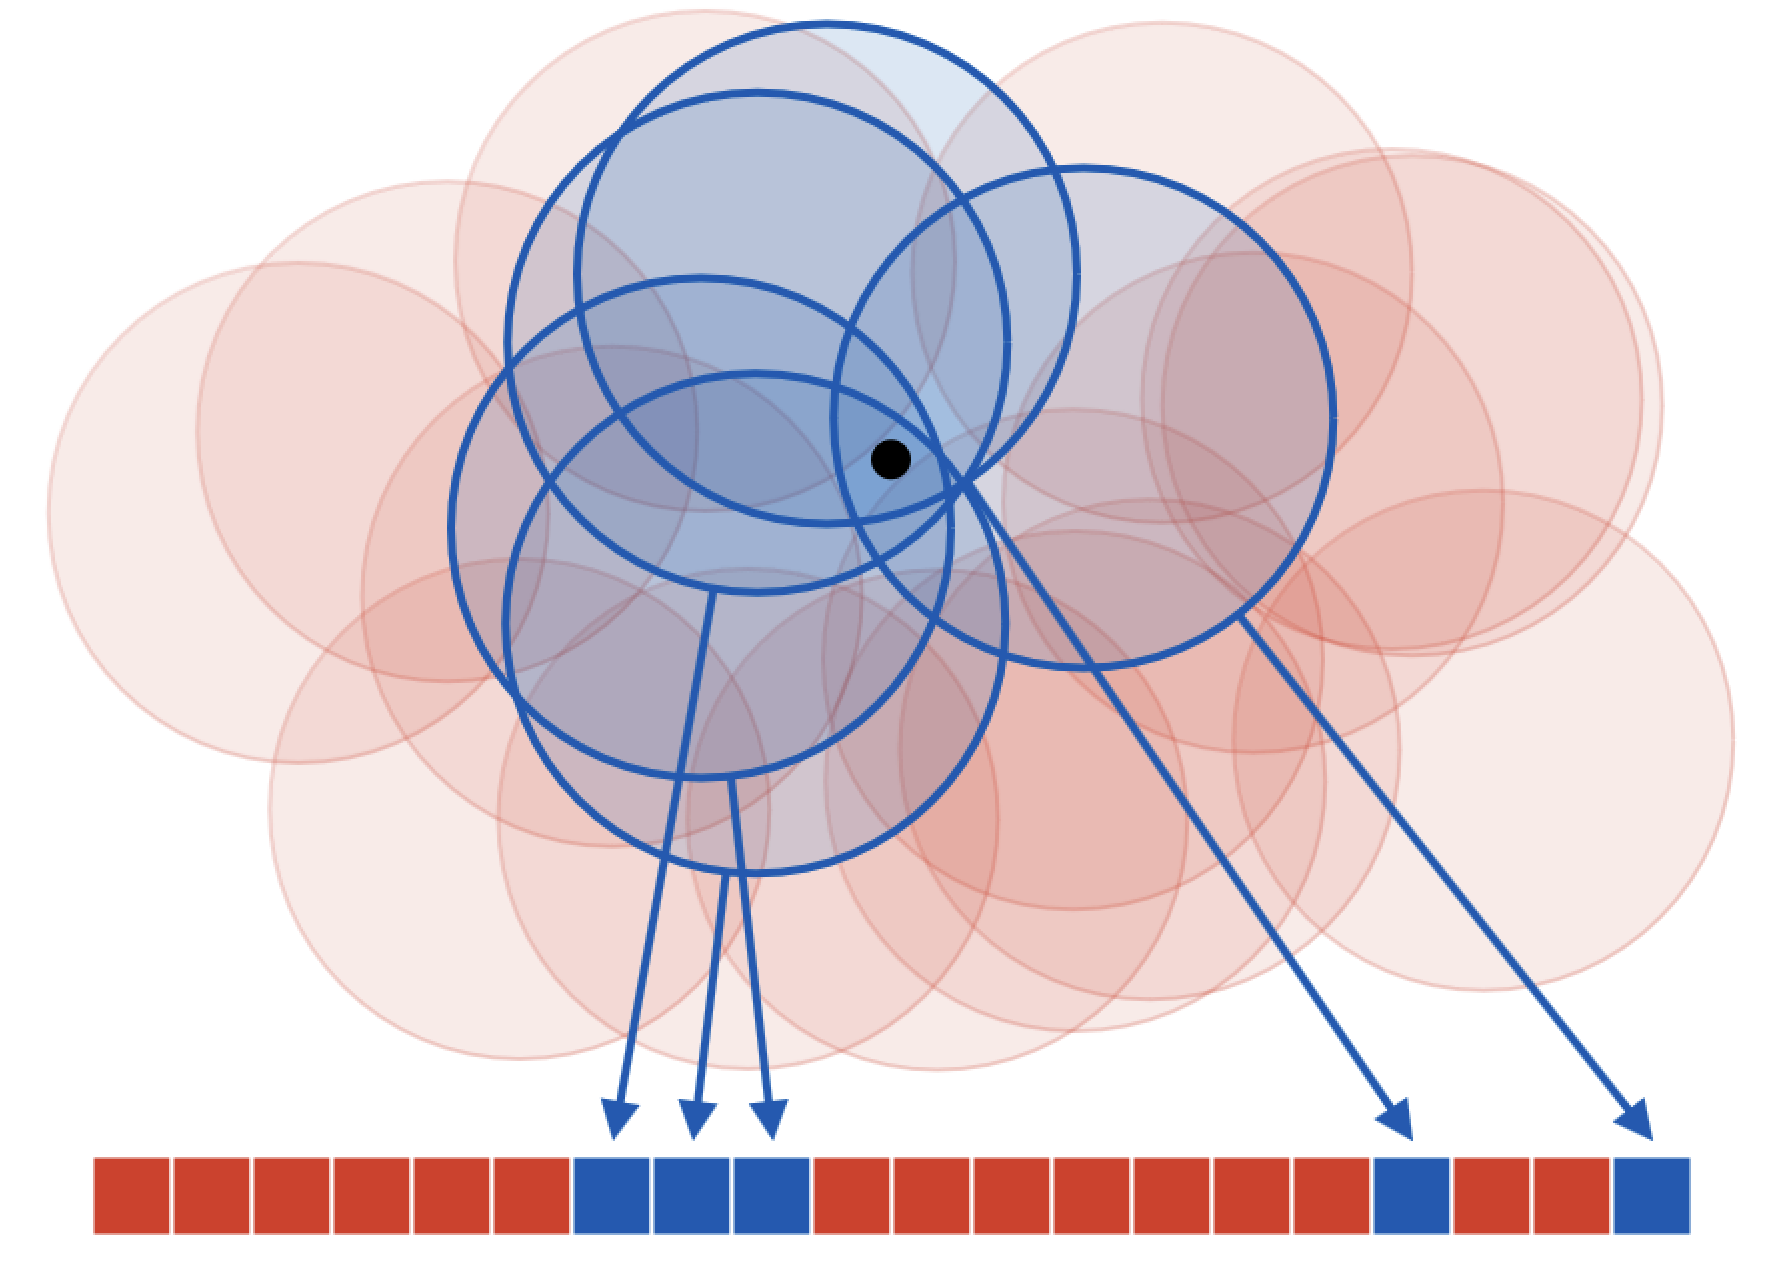
\includegraphics[width=0.8\textwidth]{../figures/coarse_code_short.png}}
				\end{center}
	\end{minipage}%
	\begin{minipage}[c]{0.5\textwidth}
		\vspace{-20pt}
		\caption{A coarse code representing a point on a plane. Each ``neuron,'' drawn as a red or blue square, encodes whether the point belongs to an associated ``receptive field.'' Although no neuron gives specific information on the position of the point, the overall code determines its position with reasonable accuracy.}
		\label{coarse-code}
	\end{minipage}
\end{figure}

If each neuron in a given neural network coded for a ``meaningful'' feature of its input, we could hope to reverse-engineer this network's overall behavior on a neuron-by-neuron basis. However, individual neurons of real-world networks often lack clear interpretations. For example, both language models and vision models have been found to learn neurons that correlate simultaneously with apparently unrelated features. (See for example \citet{nguyen_multifaceted_2016}, \citet{zhang_sample_2023} and \citet{olah_zoom_2020}.)

The difficulty of interpreting a network in terms of its local activity---and in particular, the appearance of so-called ``polysemantic neurons''---is not surprising from a connectionist viewpoint. Since at least the 1980s, proponents of neural networks have argued that these systems may naturally use \textbf{distributed representations}---coding schemes where individual features are represented by patterns spread over many neurons, and conversely where each neuron carries information on many features. (This term was apparently coined in \cite{rumelhart_parallel_1986}, Chapter 3.) In contrast, a \textit{local} representation would dedicate each neuron to a single feature. See \cite{thorpe_local_1989} for a general discussion of local and distributed codes. \Cref{coarse-code} illustrates a classic example of a coarse code, one kind of distributed representation.

As of now, relatively little is known about how deep neural networks learn to represent information in their hidden layers or to what extent this information can be interpreted. However, should ``interpretable features'' exist, the connectivist viewpoint makes it natural that they would typically be stored with non-local codes. This is a common assumption in interpretability research today; for example, when \citet{meng_locating_2022} intervened on an MLP layer of a language model to ``edit'' a factual association, both the ``subject'' and the ``fact'' were modeled as vectors of neuron activations rather than as individual neurons.

How can we infer latent features learned by a neural network? One simple proposal is to model an activation vector $x$ as a linear projection
\begin{equation*}
	x = F y \label{eq:linear-model}
\end{equation*}
of some high-dimensional and \textit{sparse} vector $y$ of latent features. We refer to the columns of $F$ as codewords and the whole matrix $F$ as a dictionary. Since $x$ is a linear superposition of codewords, we will call it a \textbf{superposition code} for $y.$ It is a remarkable fact that, for certain matrices $F,$ the linear projection $x = F y$ can code uniquely for a sparse vector $y$ even when the dimension of $x$ is (logarithmically) smaller than the dimension of $y.$ The task of inferring the sparse vector from its linear projection is known as sparse reconstruction, and the task of inferring the dictionary $F$ from a distribution over $x$ is called dictionary learning. Both of these problems have been studied in the field of compressive sensing, although with different applications in mind. (See \cite{elad_sparse_2010} for a review of classic work in the context of signal and image processing.)

Already in 2015, \cite{faruqui_sparse_2015} used a dictionary learning method to derive sparse latent codes for word embeddings and argued that these latents were more interpretable than the original embedding dimensions. More recently, a series of works beginning with \cite{yun_transformer_2021} have applied dictionary learning to the internal representations of transformer-based language models. \cite{cunningham_sparse_2023} suggested the use of \textbf{sparse autoencoders} (SAEs) and \cite{templeton_scaling_2024, gao_scaling_2024} scaled sparse autoencoders to production-size large language models.

To infer a latent representation $y \in \R^N$ from an activation vector $x \in \R^d,$ sparse autoencoders use a simple estimate of the form $\hat y(x) = \sigma(G x)$ where $G \colon \R^{N \times d}$ is some learnable matrix and $\sigma$ is a fixed ``thresholding'' operation. In \cite{gao_scaling_2024}, which is representative of large-scale sparse autoencoder applications today, $N$ was around one million and the number of non-zero coefficients $k$ in each latent vector $\hat y(x)$ was around one hundred.

\cite{templeton_scaling_2024} showed that latent features learned by SAEs are often highly intepretable, and that intervention on these features allows ``steering'' language models in predictable ways. However, as reported in \cite{gao_scaling_2024}, even SAEs with extremely large numbers of latents suffer from an apparently irreducible reconstruction error. According to \cite{sharkey_open_2025}, understanding the limitations of SAEs---and dictionary learning in general---is an important open question in the research program of mechanistic interpretability.

\subsection*{Contributions}

Over the course of computation, it is common for programs to use more memory than was required to store their input data. Similarly, it is natural to expect that the entropy of a ``simple'' (or ``interpretable'') description for the residual vectors within a language model is not bounded by the entropy of language. Methods like sparse autoencoders aim to provide descriptions of these hidden activations, but relatively little is known about the nature of the information is being carried. One basic and natural question is \textit{how much} information can hypothetically be stored in an activation vector.

In many classical situations, this question is answered by well-known ideas from information theory. Given a ``channel'' with certain characteristics---for example, a band-limited telephone connection or a binary storage device with a certain failure rate---the amount of information we can effectively transmit is asymptotically characterized by a ``channel capacity'' measured in bits per unit of channel usage. The goal of this paper is to study the carrying capacity of sparse superposition codes in a regime that is meaningful to sparse autoencoders. Our analysis focuses on a toy example, described in more detail in \Cref{sec:codes}. Our main findings are the following.

First, in an asymptotic regime of sublinear sparsity ($\ln k \le \eta \ln N$ for some $\eta < 1$), we prove that very simple ``one-step methods'' can reliably decode superposition codes when $d$ is a constant factor greater than the Shannon limit. Our asymptotic results agree very well with numerical experiments, providing good ``rules of thumb'' in practice for the top-$k$ decoder. However, we also show that the constant factor grows to infinity as $\eta$ goes to $1,$ and can already be surprisingly large for values of $(N, k)$ typical for sparse autoencoders.

Second, we show that relatively cheap iterative methods

\begin{figure}
	\begin{center}
	\begin{minipage}[]{0.63\textwidth}
		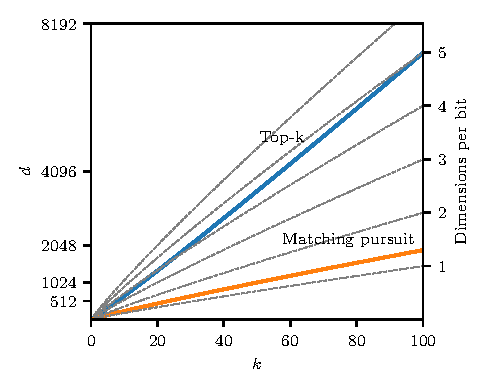
\includegraphics[width=0.95\textwidth]{../figures/storyline}
	\end{minipage}%
	\begin{minipage}[]{0.37\textwidth}
		\vspace{-29pt}\caption{An overview of the minimum codeword dimension $d$ required for two different methods to reliably decode a uniformly chosen $k$-sparse subset of $\{1, \dots, 2^{20} \}$ from a superposition of codewords from an i.i.d.\ Rademacher dictionary. The inverse ``bitrate'' $d/H(k),$ where $H(k) = \log_2 \binom N k \approx k \log_2(e N/k),$ is indicated by the right axis. Top-$k$ is a method currently used by sparse autoencoders, and matching pursuit is a relatively cheap iterative algorithm.}
		\label{fig:storyline}
	\end{minipage}
	\end{center}
\end{figure}

How ``efficient,'' in terms of bitrate, are the codes used by real neural networks? Of course, it would not make sense for a network to use a code that requires a costly iterative decoding process before it can be used. However, the success of matching pursuit suggests that neural networks may be able to improve over the bitrates of one-step estimates while paying a relatively small computational price. Although our analysis is restricted to a toy scenario, we hope these results inform future work on modeling distributed representations.

\subsection*{Related Work}

Recently, various authors have studied the underperformance of SAEs and proposed ways to improve these methods. For example, \cite{rajamanoharan_improving_2024} proposed \textit{gated SAEs} to mitigate ``feature shrinkage,'' and \cite{bussmann_learning_2025} proposed \textit{Matryoska SAEs} to deal with problems related to ``feature absorption.''

Especially relevant to this work is the proposal of \textit{inference-time optimization} (ITO), which involves replacing the encoder of an SAE with an iterative optimization method at inference time---that is, after the dictionary $F$ has already been learned. For example,  \cite{engels_decomposing_2024} evaluated gradient pursuit as an inference-time optimization method. However, if the restrictive encoders used by SAEs at training time cannot discern read certain attributes of the sparse latent signal, then the corresponding codewords will not appear in the learned dictionary. This may explain the limited improvements attained so far by ITO. We hope the present work helps clarify these questions, especially for readers who may not be familiar with ideas from compressive sensing.

\section{Superposition Codes \label{sec:codes}}

We begin by describing the toy scenario to be studied. Given a large number $N,$ consider a map $F$ that ``encodes'' each subset $y \subseteq [N] = \left\{ 1, \dots, N \right\}$ by a linear combination
$$
	x = \sum_{i \in y} f_i \in \R^d,
$$
where the vectors $\{ f_i \in \R^d : i \in [N] \}$ are chosen in advance and where the dimension $d$ of the encoding is expected to be much smaller than $N.$ We call the vectors $f_i$ codewords for the elements of $[N]$ and call the image $Fy$ a superposition code for the set $y.$ It is useful to view $y$ as a vector in $\left\{ 0, 1 \right\}^N$ with coefficients
$$
	y_i = \begin{cases}
		1: i \in y \\
		0 : \text{otherwise}
	\end{cases}
$$
and view $F$ as a matrix of column vectors $[f_1 \; \dots \; f_N],$ called the dictionary. In this work, we'll model our subset as a random variable $Y$ uniformly distributed over all subsets of some fixed size $k \ll N.$

One natural 

\begin{proposition}
	\label{prop:many-ortho}
	Let $d > 2 \epsilon^{-2} (2 \ln N + \ln p^{-1}),$ and let
	$$
		\{ F_1, \dots, F_N \} \subseteq \{ - 1/\sqrt d,  1 / \sqrt d \}^d
	$$
	be random vectors with independent, uniformly distributed entries. Then $\lvert \langle F_i, F_j \rangle \rvert < \epsilon$ for all $i \neq j$ with probability at least $(1 - p).$
\end{proposition}

We informally classify one-step methods and iterative methods. One-step methods estimate each coordinate of $Y$ using a linear function of the code $X$ and then perform a single thresholding step to refine these estimates, use One-step methods can be derived by separately considering the estimation problem for each coordinate $Y_i$
\begin{equation}
	X = Y_i f_i + \overbrace{\sum_{j \neq i} Y_j f_j}^Z \label{eq:simple-model}
\end{equation}
and approximating the sum $Z$ of other codewords as Gaussian noise. Under this simplification, it is easy to infer $Y_i$; if we model $Z$ as a centered Gaussian with non-singular covariance matrix $\Sigma$ and define an inner product by $\langle v, w \rangle_\Sigma = 1/2 x^T \Sigma^{-1} y,$ then the exact posterior of $Y_i$ conditional on $X$ is determined by the function
$$
	\lambda_i(X) = \frac{\langle f_i, X \rangle_\Sigma}{\lVert f \rVert_\Sigma^2}.
$$
In signal processing, this kind of linear measurement is called a \textbf{matched filter} for the codeword $f_i$. The log odds of the posterior on $Y_i$ in terms of the matched filter is given by
\begin{align} \label{eq:log_odds}
	 & \ln \frac{\Pp(Y_i = 1|X = x)}{\Pp(Y_i = 0|X = x)} \nonumber                         \\
	 & = \rho \left(\lambda(x) - \frac 1 2\right) + \ln \frac{\Pp(Y_i = 1)}{\Pp(Y_i = 0)},
\end{align}
where $\rho = \lVert f \rVert_\Sigma^2$ is called the ``signal-to-noise ratio'' of the filter $\lambda.$ See \Cref{appendix:matched} for a review.

When the number $k$ of non-zero coefficients is known, it is also natural to set $\hat{Y}_i = 1$ for the $k$ indices $i$ with maximum matched filters. This is called top-$k$ decoding. \cite{gao_scaling_2024} showed that, in practice, top-$k$ autoencoders perform better than their ReLU variants in practice.

The second class are the iterative methods.

We're interested in understanding how large the dimension $d$ needs to be as a function of $(N, k)$ for a given inference method to recover $Y.$ (We do not study the problem of learning the dictionary.) Since $Y$ is a discrete variable, we will focus on conditions for \textit{exact} recovery. We focus on a regime where $Y$ resembles the very sparse latent representations learned by sparse autoencoders trained on large language models. For example, typical values discussed in \cite{gao_scaling_2024} are $N = 2^{6}$ and $k = 100.$

% In the following, let us assume that the codewords $f_i \in \R^d$ are unit vectors. (It is natural for all the codewords $f_i$ to have the same magnitude if each coefficient $Y_i$ needs to be encoded with the same precision, as they do in our scenario.) If we assume further that the empirical distribution over codewords $f_i$ is approximately isotropic, then the matched filter for $Y_i$ is approximately
% $$
% 	\lambda_i(X) = \langle f_i, X \rangle.
% $$
% (If the distribution over codewords is not isotropic, we can first apply a linear transformation to ``whiten'' the distribution of $X.$)

% A \textbf{one-step estimate} is an estimate for $Y$ that relies directly on the matched filters $\lambda_i.$ From \Cref{eq:log_odds}, the maximum likelihood estimate for $Y_i$ under our simplified Gaussian model is $1$ if
% $$
% 	\langle f_i, X \rangle \ge \frac 1 \rho \ln \frac {\Pp(Y_i = 1)} {\Pp(Y_i = 0)} + \frac 1 2
% $$
% and $0$ otherwise. If we assume the signal-to-noise ratio $\rho$ is very large, the decision boundary becomes approximately $1/2.$ This leads to the simpler of the two one-step estimates that we will consider.
% \begin{definition}
% 	Given $X = FY,$ the \textbf{threshold decoding} is
% 	$$
% 		\hat{Y}_i = \begin{cases}
% 			1 : \langle f_i, X \rangle \ge 1/2 \\
% 			0 : \text{otherwise.}
% 		\end{cases}
% 	$$
% \end{definition}

% On the other hand, if we know (or guess) the size $k$ of the set $Y$ in advance, the following is a natural way to make use of that information. (In the context of sparse autoencoders, this method was introduced by \cite{makhzani_k-sparse_2014}.)

% \begin{definition}
% 	Given $X = F Y,$ the \textbf{top-$k$ decoding} is the set $\hat Y$ of $k$ elements whose codewords $f_i$ have largest inner products with $X.$ (Ties are broken arbitrarily.)
% \end{definition}

% Note that whenever threshold decoding succeeds at recovering $Y,$ top-$k$ decoding succeeds as well. Indeed, top-$k$ decoding can be viewed as a kind of threshold decoding where the threshold is chosen optimally as a function of $X.$

\section{Information Theory Bounds \label{sec:information}}

We recall the idea of channel capacity with a simple example. Suppose that the latent variable $Y$ to be encoded is a symbol drawn from an alphabet of size $N.$ What is the minimum dimension $d$ such that each value of $Y$ can be represented by a vector $X \in \R^d$?

When the vector $X$ can be stored exactly, the answer to our question simply depends on the number of values it can take. If the coefficients of $X$ are $16$ bit floating point numbers, then each coefficient can store (nearly) $2^{16}$ distinct numbers, and overall we need only about $d_\text{min} \approx \frac 1 {16} \log_2 N$ dimensions.

However, we expect that activation vectors within real neural networks are subject to various kinds of interference. For example, an activation vector $X$ may need to represent the symbol $Y$ while also holding information on another latent quantity, or it may be subject to explicitly induced noise like dropout. Characterizing the ``capacity'' of a vector in the presence of interference is a basic problem in coding theory.

One common model is to consider that $X$ is subject to additive white Gaussian noise. More specifically, we let $Z \in \R^d$ be a vector of independent, centered Gaussians each of variance $P,$ and consider the problem of recovering $Y$ from $X + Z.$ The following is then a typical (but remarkable) result of information theory.

\begin{proposition} \label{prop:information}
    Let the random variable $Y \in [N]$ be uniformly distributed, and let $Z$ be white Gaussian noise of variance $P.$ Suppose there exist a pair of maps $F \colon [N] \to \R^d$ and $G \colon \R^d \to [N]$ so that
	$$
		G(F(Y) + Z) = Y
	$$
	with probability at least $(1 - p),$ and suppose the variance of each coordinate of $F(Y)$ is bounded by $1.$ Then
	$$
	d \geq 2 \frac{(1 - p) \ln N - \ln 2}{\ln \bigl( 1 + P^{-1} \bigr)}.
	$$
\end{proposition}

In particular, if we fix $P$ and let the number $N$ of symbols grow to infinity, this shows that the minimum dimension $d$ of a reliable code must grow logarithmically in $N.$ More specifically, we can say the following.

\begin{corollary} \label{prop:information-simple}
    Fix $P > 0,$ $\epsilon > 0,$ and suppose
    $$
    d \le \left(\frac 2 {\ln(1 + P^{-1})} - \epsilon\right) \ln N.
    $$
    Then, when the random variables $(Y, Z)$ and the maps $(F, G)$ are in the conditions of \Cref{prop:information}, the maximum value of $\Pp(G(F(Y) + Z) = Y)$ converges to $0$ for sufficiently large $N.$
\end{corollary}

Since $\ln(1 + P^{-1})^{-1} \approx P$ for large $P,$ this means that roughly $d \ge 2 P \ln N$ dimensions are needed to reliably code for $Y.$

Now, one very simple way to construct maps $F$ and $G$ is to choose the codewords $F(i)$ randomly from some distribution on the unit sphere in $\R^d$ and let $G(v)$ return the element $j$ so that $\langle v, F(j) \rangle$ is maximized. For brevity, we refer to $(F, G)$ This strategy can be motivated by the remarkable fact that random codebooks of size $\Omega(e^d)$ of $d$-dimensional codewords can have bounded interference, in the sense of the following result.

\begin{proposition} \label{prop:random-information}
    Let $(F, G)$ be constructed according to the random codebook strategy, let $\epsilon > 0,$ and let
    $$
    d \ge (2 + \epsilon) P \ln N.
    $$
    Then, when the random variable $(Y, Z)$ are in the conditions of \Cref{prop:information}, $\Pp(G(F(Y) + Z) = Y)$ converges to $1$ for large $N.$
\end{proposition}

Altogether, this shows that transmitting

% \begin{figure}
% 	\begin{minipage}[c]{0.5\textwidth}
% 	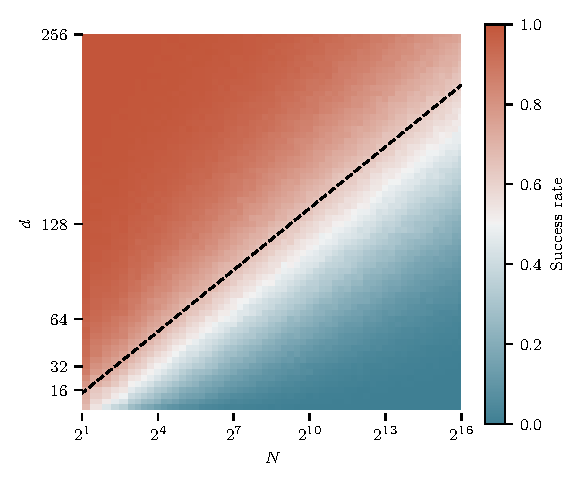
\includegraphics[width=\textwidth]{../figures/symbol_transmission}
% 	\end{minipage}%
% 	\begin{minipage}[c]{0.5\textwidth}
% 	\vspace{20pt}
% 	\caption{How many dimensions $d$ does the vector $X \in \R^d$ need to have for $X + Z$ to reliably code for an element $Y \in [N]$? This figure shows empirical success of the random codebook strategy when $Z$ is white noise with components of power $P.$}
% 	\label{fig:transmission}
% 	\end{minipage}
% \end{figure}

Our discussion so far parallels many \cite{cover_elements_2006}. In the remainder of this work, we consider

It will also be useful to know the upper bound
$$
	H = \ln \binom N k \le k \ln (eN/k) = k \ln N - k \ln k + k
$$
on the entropy of a random $k$-element subset of $[N],$ which turns out to be a very good approximation when $k \ll N.$ For example, when $N = 2^{20}$ and $k = 2^8,$ the approximation
$$
	\ln \binom{2^{20}}{2^8} \approx 2^8 \ln(2^{20} e/2^8) = 128 (1 + 12 \ln 2)
$$
holds with a relative error of only about $0.3 \%.$ (See \Cref{appendix:binomial} for a discussion of this estimate.)

\subsection{Results for Random Dictionaries \label{sec:random-results}}

\begin{figure}
	\begin{center}
	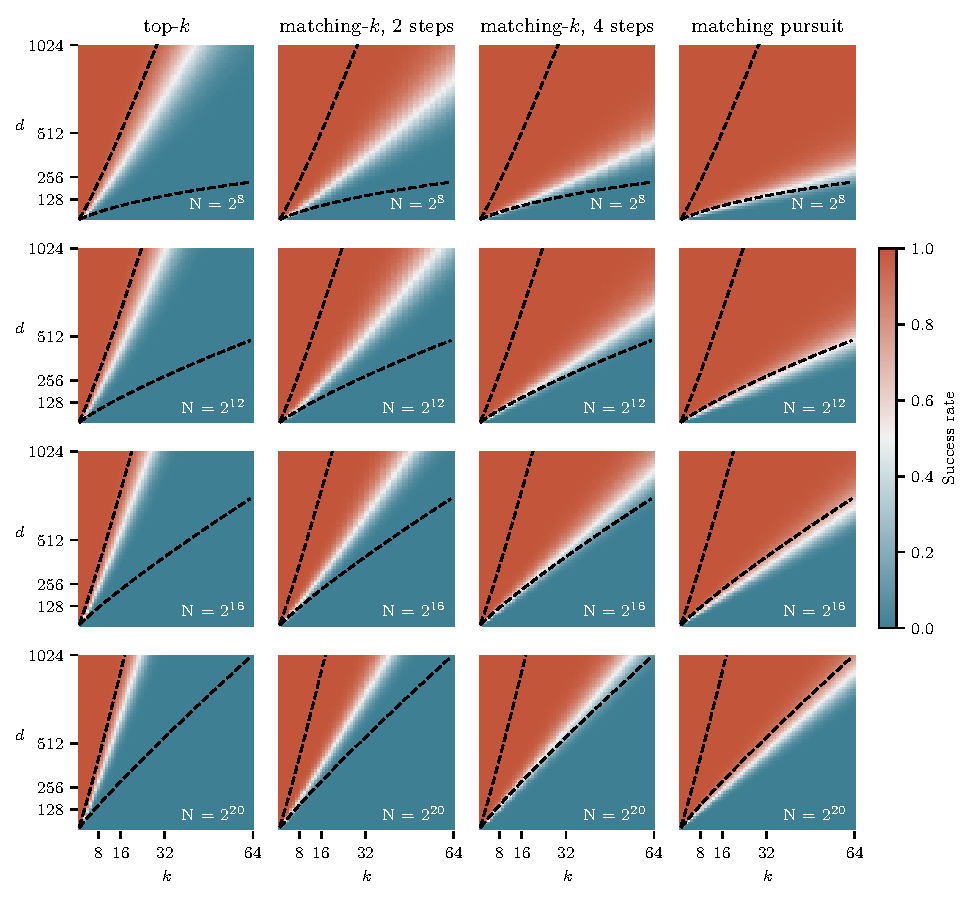
\includegraphics[width=\textwidth]{../figures/pursuit}
	\caption{Empirical performance of a variety of different decoding methods at reading a $k$-element subset of $[N]$ from a $d$-dimensional superposition code with a Rademacher dictionary.}
	\label{fig:pursuit}
	\end{center}
\end{figure}

\begin{figure}
	\begin{center}
	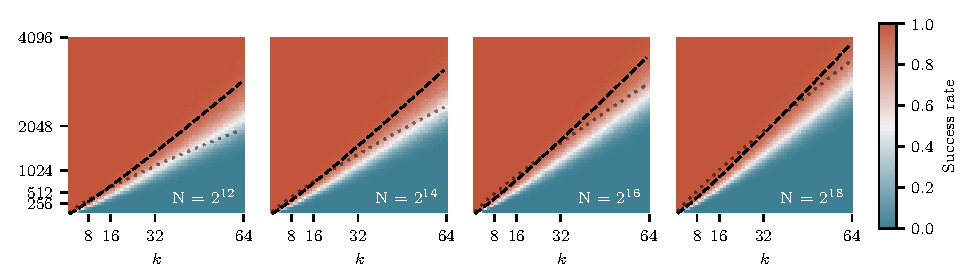
\includegraphics[width=\textwidth]{../figures/top_k}
	\caption{The prediciton of Proposition \Cref{prop:sufficient-cond} agrees well with numerical experiments.}
	\label{fig:top-k}
	\end{center}
\end{figure}

\begin{figure}
	\begin{center}
	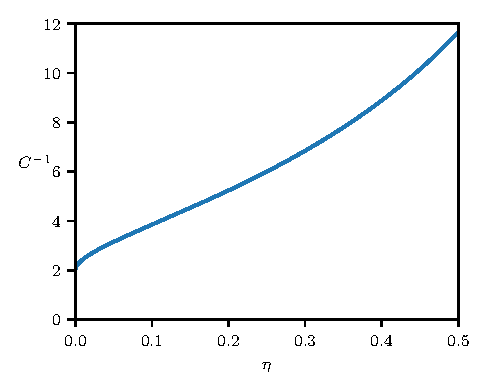
\includegraphics[width=0.5 \textwidth]{../figures/capacity}
	\caption{Inverse channel capacity (in nats per dimension) predicted by \Cref{prop:sufficient-cond}.}
	\label{fig:capacity}
	\end{center}
\end{figure}

Our first result on random dictionaries provides an

\begin{proposition} \label{prop:necessary-cond}
    Let $F$ and $G$ be as above, and let $C < 2.$ Then for sufficiently large $N,$ $\Pp(G(F(Y)) = Y) < 1/2.$
\end{proposition}

This shows that

\begin{proposition} \label{prop:sufficient-cond}
	For $\epsilon \in (0, 1),$ let $\ln k \le \epsilon \ln N,$ and let
	$$
	\kappa > 2 + 4 \sqrt \epsilon + 2 \epsilon.
	$$
	Suppose $d \ge \kappa \ln N.$ Then for sufficiently large $N,$ $G(F(Y)) = Y$ with arbitrarily high probability.
\end{proposition}

Since
$$
2 + 4 \sqrt \epsilon + 2 \epsilon \le 4(1  + \epsilon)
$$
and when $k = N^\epsilon,$ $4(1 + \epsilon) k \ln N = 4 k \ln (N / k),$ \Cref{prop:sufficient-cond} shows that.

This predictions agrees well with numerical experiments, graphed in \Cref{fig:one-step}. In fact, even as $N$ varies over several orders of magnitude, the slightly weaker condition $d \ge 8 k \ln N$ characterizes the regime where the set $Y$ can be decoded with reasonably high probability by threshold decoding.

Top-$k$ decoding performs significantly better but admits a similar ``rule of thumb'': for all values of $N$ trialed, $d = 4 k \ln k N$ is very close to the smallest dimension needed for top-$k$ decoding to succeed with high probability. See \Cref{appendix:top_k} for an informal derivation of this bound.

There are several ways to interpret this conclusion. On one hand, it means that one-step estimates are asymptotically ``inefficient'' in terms of required bitrate when $k$ is moderately large compared to $N.$ More specifically, in a regime where $N$ goes to infinity but $\ln k / \ln N$ converges to $1,$ we predict that one-step estimates require the ratio $d/H$ to diverge to infinity.

In particular, one-step estimates are asymptotically inefficient when $k/N \ge \epsilon$ for some positive $\epsilon.$ Indeed, to have $d \ge 4 k \ln N$ in this case we would need $d = \Omega(N \ln(N)),$ while the entropy of $Y$ is only $O(N).$ In contrast, a hallmark result of compressive sensing implies that, when $k/N \le \epsilon,$ the vector $y$ can be recovered from its image $F y$ under a random projection by a certain \textit{convex} optimization problem so long as $d \ge \kappa(\epsilon) N$ for some constant $\kappa(\epsilon)$; for example, see \cite{candes_decoding_2005}. The failure of our one-step estimates in this particular regime is easy to prove.

On the other hand, in a sparser regime where $\ln k / \ln N < \epsilon$ for some $\epsilon < 1,$ it follows from our analysis that one-step estimates are ``information-efficient'' in the sense that they can be decoded from superposition codes that achieve bitrates $H/d$ larger than some positive $\delta.$ However, it is also of interest to have \textit{non-asymptotic} information on the required bitrate. From \Cref{eq:bitrate} we find that one-step estimates need at least $4 \ln 2 \approx 2.8$ bits per dimension even for small $k.$ When $k = 2^8$ and $N = 2^{20}$ this number rises to about $4.1,$ and the experiments of \Cref{fig:one-step} show that this factor is in fact slightly optimistic. If we use threshold decoding instead of top-$k,$ we need $8$ dimensions per bit! Can other inference algorithms do significantly better?

There is an extensive literature on theory of compressive sensing. \cite{reeves_all-or-nothing_2019} shows that, in our language, superposition codes with a random dictionary are essentially optimal in the information-theoretic sense when ideal maximum-likelihood inference is used as the decoder. A series of earlier works (\cite{joseph_least_2012, joseph_fast_2014, rush_capacity-achieving_2017}) on superposition codes also showed that, under some special conditions on $y$, certain decoding schemes admit bitrates up to theoretical channel capacity in the presence of Gaussian noise. However, to our knowledge, practical guarantees on the performance of iterative methods are not available for our range of $k$ and $N.$

\Cref{fig:mp} shows the results of a numerical experiment using an iterative method called \textit{matching pursuit}, first suggested in \cite{bergeaud_matching_1995}. This is a simple ``greedy'' algorithm that initializes $y = 0$ and, at each of $k$ iterations, increments the index of $y$ whose corresponding codeword has largest inner product with $x - Fy.$

Matching pursuit far outperforms top-$k$ decoding for the range of $N$ and $k$ considered earlier. When $d \ge 1.3 \log_2 (e N /k)$ and $N > 2^{16},$ our experiments show that matching pursuit is very reliable. In other words, matching pursuit can reliably infer a sparse vector from just $1.3$ dimensions per bit. In \Cref{appendix:bp} we find that a more computationally expensive algorithm called basis pursuit can do slightly better, requiring only 0.8 dimensions per bit.


\bibliography{capacity_paper}
\bibliographystyle{tmlr}

% \appendix
% \section{Appendix}
% \input{content/100_appendix_information}
% \input{content/100_appendix_bp}
% \input{content/100_appendix_proofs}
% \input{content/100_appendix_simple_jl}

\end{document}
